\documentclass[12pt,a4paper]{article}

\usepackage[utf8]{inputenc}
\usepackage[T1]{fontenc}
\usepackage{graphicx}
\usepackage{amsmath}
\usepackage{amssymb}
\usepackage{geometry}
\usepackage{fancyhdr}
\usepackage{enumitem}
\usepackage{parskip}
\usepackage{xcolor}
\usepackage{anyfontsize}
\usepackage{subcaption}
\usepackage{booktabs}
\usepackage{array}
\usepackage{siunitx}
\usepackage{setspace}
\usepackage[colorlinks=true]{hyperref}
\usepackage{float}
\usepackage{tabularx}
\usepackage{longtable}
\usepackage{makecell}
\usepackage{caption}
\usepackage{adjustbox}
\usepackage{placeins}

\onehalfspacing

% =====================================
% Colors and Styles
% =====================================
\definecolor{itiBlue}{RGB}{0,82,147}
\definecolor{absblack}{RGB}{0,0,0}
\definecolor{lightBlue}{RGB}{236,244,250}

\hypersetup{
    linkcolor = absblack,
    urlcolor = itiBlue,
    citecolor = itiBlue,
    allbordercolors = {0 0 0},
    pdfborder = {0 0 0}
}

% =====================================
% Page Layout
% =====================================
\geometry{a4paper, margin=1in}
\setlength{\parindent}{0pt}
\setlength{\parskip}{6pt}
\setlength{\headheight}{15pt}
\emergencystretch=2em
\sisetup{group-separator={,},group-minimum-digits=4}
\captionsetup{font=small,labelfont=bf}
\captionsetup[table]{skip=6pt}
\captionsetup[figure]{skip=6pt}

\pagestyle{fancy}
\fancyhf{}

\rhead{Project 6 Weekly Radar Report}
\lhead{\thepage}
\renewcommand{\headrulewidth}{0.4pt}

\fancyfoot[C]{%
    \vspace{5pt}%
    \rule{\textwidth}{0.4pt}\\%
    \vspace{2pt}%
    \thepage%
}

\newcommand{\keyterm}[1]{\textbf{#1}}

\begin{document}

    \begin{titlepage}
        \centering

        \begin{figure}[htbp]
            \centering
            
\includegraphics[width=0.72\linewidth]{Images/ITI_Logo.png}
        \end{figure}

        \vspace{0.8cm}

        \textcolor{absblack}{\rule{1\textwidth}{1.5pt}} \\[0.8cm]

        {\fontsize{21}{28}\selectfont\bfseries Project 6 Report: Weekly Radar}\\[0.4cm]
        {\fontsize{16}{18}\selectfont\bfseries Anomaly Detection on Weekly Network Performance}\\[0.25cm]
        {\fontsize{13}{16}\selectfont\bfseries Carrier and Region Trend Analysis for Egyptian Governorates}

        \textcolor{absblack}{\rule{1\textwidth}{1.5pt}} \\[1.3cm]

        \vspace*{0.6cm}

        {\renewcommand{\arraystretch}{1.4}
        \begin{tabular}{@{}p{5cm}p{8.5cm}@{}}
            \textbf{\large Submitted by:} & \large Osama Mohamed Eglal \\[0.15cm]
            & \normalsize \textcolor{itiBlue}{\href{mailto:osamaeglal143@gmail.com}{osamaeglal143@gmail.com}} \\[0.15cm]
            & \normalsize Intake 46 \\[0.55cm]
            \textbf{\large Submitted to:} & \large Ibrahim H. El-Shal \\[0.55cm]
            \textbf{\large Date:} & \large \today \\
        \end{tabular}
        }

        \vfill

        \textcolor{absblack}{\rule{1\textwidth}{1pt}}

        \thispagestyle{empty}
    \end{titlepage}

    \tableofcontents
    \newpage

\section{Introduction}

This report documents the final corrected workflow for \textbf{Project 6 --- Weekly Radar} from the ITI Telco-Cloud Analytics training. The project analyzes weekly mobile network performance across Egyptian governorates, carriers, and radio technologies.

The workflow has two main notebook phases:

\begin{enumerate}[label=\arabic*.]
    \item a \textbf{preprocessing notebook} that cleaned the original workbook, separated weekly locality rows from country aggregates, and built the final region-carrier-technology-week table; and
    \item an \textbf{analysis notebook} that applied cross-sectional peer comparison, week-over-week change analysis, LTE-vs-5G comparison, regional ranking, and mean-vs-median interpretation.
\end{enumerate}

The key analytical challenge is that the weekly dataset contains only three weekly snapshots: 2026-03-01, 2026-03-08, and 2026-03-15. Therefore, the project is not a long-history time-series anomaly problem. The strongest approach is to compare entities that exist at the same time: carriers against same-region peers, regions against other regions, and technologies across matched region-week records.

\section{Project Objective and Analytical Design}

The project brief asks five main questions:

\begin{enumerate}[label=\textbf{Q\arabic*.}]
    \item Which carriers are consistently below the regional average for download speed across all three weeks?
    \item Which regions show the largest week-over-week change in download speed or latency?
    \item Are there region-carrier pairs that are outliers inside their region?
    \item Is the 5G performance distribution different from LTE across regions?
    \item How do the 13 regions rank from best to worst based on median download speed, and which region has the most unstable rank?
\end{enumerate}

The final design used the following principles:

\begin{itemize}
    \item \textbf{Weighted aggregation:} KPI values were aggregated using \texttt{sample\_count} as reliability weight.
    \item \textbf{Median proxy:} regional median KPI columns are sample-count-weighted averages of locality medians. They are strong proxies, but not exact combined medians because raw speed-test observations are not available.
    \item \textbf{Reliability threshold:} the final preprocessing threshold was reduced from 50 to \texttt{sample\_count\_total >= 30} to preserve full region-week coverage while still filtering weak records.
    \item \textbf{Complete peer groups:} Q1 and Q3 use only region-week-technology groups where all three carriers exist, making peer comparisons fair.
    \item \textbf{Interpretability:} every anomaly score is tied back to a named region, carrier, technology, week, and KPI direction.
\end{itemize}

\section{Preprocessing Notebook}

\subsection{Why preprocessing was necessary}

The original spreadsheet mixed daily and weekly rows, locality and country rows, and many repeated locality records that had to be aggregated into a clean project-level unit. The final analysis unit is:

\[
\text{region} \times \text{carrier} \times \text{technology} \times \text{week}
\]

\begin{table}[htbp]
\centering
\begin{adjustbox}{max width=\textwidth}
\begin{tabular}{p{9cm}r}
\toprule
Processing stage & Rows \\
\midrule
Raw spreadsheet rows & 93,364 \\
Weekly rows kept & 58,858 \\
Daily rows removed & 34,506 \\
Weekly locality rows & 58,669 \\
Weekly country rows & 189 \\
Aggregated region-carrier-technology-week rows & 351 \\
Rows removed by sample threshold & 8 \\
Final analysis rows & 343 \\
\bottomrule
\end{tabular}
\end{adjustbox}
\caption{Row counts through the corrected preprocessing pipeline.}
\label{tab:preprocess}
\end{table}

Table~\ref{tab:preprocess} shows the corrected pipeline. The workbook started with \num{93364} rows. After weekly filtering, \num{58858} rows remained. Locality rows were used for the main region-level analysis, while 189 Egypt-level country aggregates were separated as optional reference rows. After region-carrier-technology-week aggregation, 351 rows existed before reliability filtering. The threshold \texttt{sample\_count\_total >= 30} removed only 8 weak rows and left 343 final rows.

\subsection{Date parsing and validation}

One important correction was the date parser. The final notebooks avoid forcing \texttt{dayfirst=True} on already-standard ISO dates such as \texttt{2026-03-15}. This prevents the third week from being converted incorrectly or dropped. The corrected validation confirms that all three weekly snapshots are present.

\begin{table}[htbp]
\centering
\begin{adjustbox}{max width=\textwidth}
\begin{tabular}{p{8cm}p{6cm}}
\toprule
Validation check & Final result \\
\midrule
Main cleaned table & 343 region-carrier-technology-week rows \\
Weeks present & 3 / 3 \\
Regions present & 13 / 13 \\
Region-week coverage & 39 / 39 \\
Region-technology-week coverage & 117 / 117 \\
Region-carrier-week coverage & 117 / 117 \\
Rows used for complete peer comparison & 330 \\
Rows excluded from peer comparison & 13 \\
\bottomrule
\end{tabular}
\end{adjustbox}
\caption{Final coverage checks after applying the threshold of \texttt{sample\_count\_total >= 30}.}
\label{tab:coverage}
\end{table}

\subsection{Why aggregation and weighting were required}

The locality-level rows are not strong enough individually. Many locality rows contain very small sample counts, while the aggregated regional records are much more reliable. Therefore, each KPI was aggregated with:

\[
\bar{x}_w = \frac{\sum_i x_i \cdot n_i}{\sum_i n_i}
\]

where \(x_i\) is the KPI value and \(n_i\) is the \texttt{sample\_count} behind that locality record.

\begin{table}[htbp]
\centering
\begin{adjustbox}{max width=\textwidth}
\begin{tabular}{lrrrr}
\toprule
Dataset & Median & Mean & Min & Max \\
\midrule
Weekly locality rows & 2 & 23.00 & 1 & 6,732 \\
Aggregated rows before threshold & 972 & 3,844.27 & 8 & 38,163 \\
Final rows after threshold & 1,009 & 3,933.50 & 30 & 38,163 \\
\bottomrule
\end{tabular}
\end{adjustbox}
\caption{Sample-count quality before and after region-level aggregation.}
\label{tab:sample}
\end{table}

The locality-level weekly rows had a median sample count of only 2, while the final filtered region-level rows had a median sample count of \num{1009}. This is why the weighted aggregation step is not just a coding detail; it is part of the reliability design.

\section{Analysis Notebook: Methods}

\subsection{Threshold audit}

The final notebooks use a small number of threshold-like decisions. Table~\ref{tab:thresholds} summarizes each one and why it is appropriate.

\begin{table}[htbp]
\centering
\small
\begin{adjustbox}{max width=\textwidth}
\begin{tabular}{p{4.1cm}p{4.0cm}p{7cm}}
\toprule
Decision & Value & Reason \\
\midrule
Preprocessing sample threshold & \texttt{sample\_count\_total >= 30} & Keeps all 39 region-week combinations while removing only the weakest 8 aggregated rows. \\
Complete peer-group rule & exactly 3 carriers & Ensures Q1 and Q3 compare carriers only against complete same-region, same-week, same-technology peer groups. \\
Peer anomaly cutoff & 95th percentile = 84.89 & Keeps the most severe cross-sectional cases from 330 comparable rows. \\
Week-over-week anomaly cutoff & 90th percentile = 1.319 & Less brittle than 95th percentile because only 26 region transition rows exist. \\
Q2 reporting list & \texttt{TOP\_N = 5} & Readable reporting rule for largest download drops and latency rises; not a statistical anomaly threshold. \\
\bottomrule
\end{tabular}
\end{adjustbox}
\caption{Threshold audit used in the final preprocessing and analysis notebooks.}
\label{tab:thresholds}
\end{table}

\subsection{Method 1: Cross-sectional peer comparison}

For each \texttt{region $\times$ week $\times$ technology} group, each carrier was compared against the weighted average of the other carriers in that same peer group.

\[
\text{Download Gap (\%)} =
\frac{\text{Carrier Download} - \text{Peer Average Download}}{\text{Peer Average Download}} \times 100
\]

\[
\text{Latency Gap (\%)} =
\frac{\text{Carrier Latency} - \text{Peer Average Latency}}{\text{Peer Average Latency}} \times 100
\]

A negative download gap is bad because the carrier is slower than peers. A positive latency gap is bad because the carrier is more latent than peers. The final peer anomaly score follows the same formula used in the slides:

\[
\text{Cross-sectional Badness} =
\max(0, -\text{Download Gap (\%)}) + \max(0, \text{Latency Gap (\%)})
\]

The score is measured in combined bad percentage-gap points. For example, a row with download 60\% below peers and latency 30\% above peers receives a score of 90.

\subsection{Method 2: Week-over-week regional change analysis}

The second method identifies regional changes between consecutive weeks. Carrier and technology rows were combined into one weighted regional summary per week. Then the following equation was applied:

\[
\text{WoW Change (\%)} =
\frac{\text{Current Week KPI} - \text{Previous Week KPI}}{\text{Previous Week KPI}} \times 100
\]

Large negative download changes and large positive latency changes were treated as deterioration signals. The analysis also keeps direct-answer tables for the largest download drops and the largest latency rises, because a region can deteriorate in only one KPI.

\section{Results and Discussion}

\subsection{Q1: Which carriers are consistently below the regional average?}

The corrected Q1 result is more nuanced than the first report version. \textbf{Operator C} is still the main consistent underperformer because it has the strongest negative download gap, the highest weighted below-peer rate, and 16 of the 17 severe peer anomaly flags. \textbf{Operator B} is slightly below the weighted peer baseline across the three weeks, but its gap is small and almost neutral by 2026-03-15. \textbf{Operator A} remains clearly above peers overall.

\begin{table}[htbp]
\centering
\scriptsize
\begin{adjustbox}{max width=\textwidth}
\begin{tabular}{lrrrrrrp{3.5cm}}
\toprule
Carrier & 2026-03-01 gap & 2026-03-08 gap & 2026-03-15 gap & Overall gap & Below-peer rate & Flags & Interpretation \\
\midrule
Operator A & 29.94 & 28.66 & 27.08 & 28.57 & 48.0\% & 0 & Above peers overall \\
Operator B & -5.54 & -4.73 & -0.06 & -3.54 & 50.6\% & 1 & Slightly below; near neutral by week 3 \\
Operator C & -12.13 & -6.92 & -13.58 & -10.81 & 63.5\% & 16 & Main consistent underperformer \\
\bottomrule
\end{tabular}
\end{adjustbox}
\caption{Carrier download gap relative to the weighted regional peer baseline. Gaps are percentages; negative values mean below peers.}
\label{tab:carrier}
\end{table}

\begin{figure}[htbp]
    \centering
    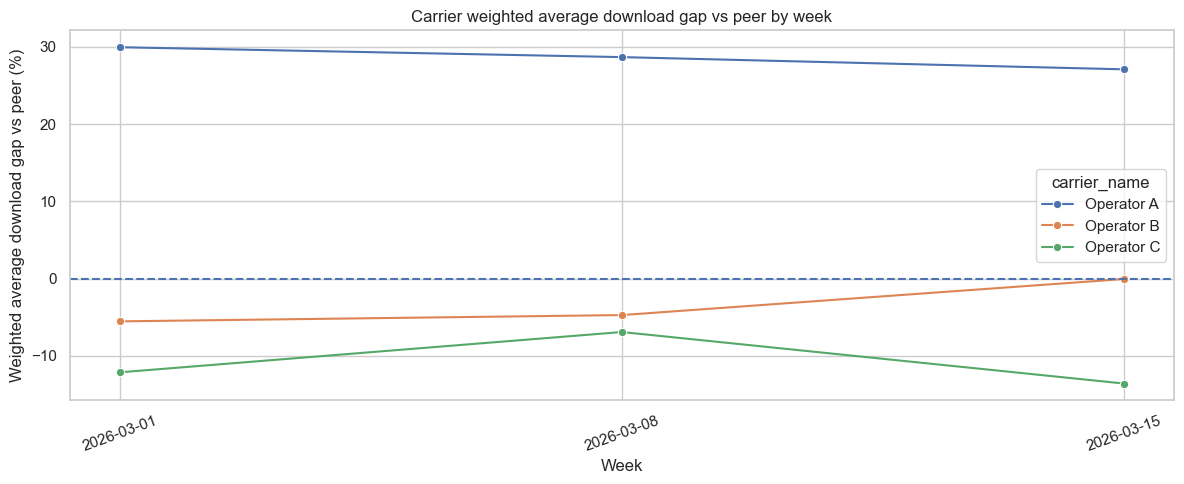
\includegraphics[width=1\linewidth]{Images/carrier_download_gap_by_week.png}
    \caption{Weighted average carrier download gap relative to regional peers by week.}
    \label{fig:carriergap}
\end{figure}

\FloatBarrier

\subsection{Q2: Which regions had the largest week-over-week changes?}

The largest \textbf{download deterioration} cases are shown in Table~\ref{tab:dlchg}. These are direct download drops, not necessarily combined download-and-latency anomaly flags.

\begin{table}[htbp]
\centering
\small
\begin{adjustbox}{max width=\textwidth}
\begin{tabular}{l l r r}
\toprule
Week & Region & Download change (\%) & Latency change (\%) \\
\midrule
2026-03-15 & Assiut & -14.54 & -0.04 \\
2026-03-15 & Monufia & -13.31 & 1.27 \\
2026-03-15 & Gharbia & -13.29 & 2.19 \\
2026-03-15 & Minya & -12.96 & 2.22 \\
2026-03-08 & Alexandria & -12.93 & -1.29 \\
\bottomrule
\end{tabular}
\end{adjustbox}
\caption{Largest negative week-over-week download changes.}
\label{tab:dlchg}
\end{table}

The largest \textbf{latency deterioration} cases are shown in Table~\ref{tab:latchg}.

\begin{table}[htbp]
\centering
\small
\begin{adjustbox}{max width=\textwidth}
\begin{tabular}{l l r r}
\toprule
Week & Region & Download change (\%) & Latency change (\%) \\
\midrule
2026-03-08 & Monufia & 9.78 & 4.85 \\
2026-03-15 & Sohag & 9.55 & 4.73 \\
2026-03-15 & Dakahlia & -6.33 & 4.08 \\
2026-03-15 & Fayoum & 9.74 & 3.24 \\
2026-03-08 & Sharqia & -0.15 & 3.10 \\
\bottomrule
\end{tabular}
\end{adjustbox}
\caption{Largest positive week-over-week latency changes.}
\label{tab:latchg}
\end{table}

The combined week-over-week anomaly score is useful when both directions are considered together. The top combined cases are shown in Table~\ref{tab:combinedwow} and Figure~\ref{fig:combinedwow}. Dakahlia appears twice because it had both download decline and latency increase across consecutive transitions.

\begin{table}[htbp]
\centering
\small
\begin{adjustbox}{max width=\textwidth}
\begin{tabular}{l l r r r c}
\toprule
Week & Region & Download change (\%) & Latency change (\%) & Combined score & Flagged? \\
\midrule
2026-03-08 & Dakahlia & -10.98 & 2.86 & 1.611 & Yes \\
2026-03-15 & Dakahlia & -6.33 & 4.08 & 1.389 & Yes \\
2026-03-08 & Port Said & -7.34 & 2.70 & 1.333 & Yes \\
2026-03-15 & Gharbia & -13.29 & 2.19 & 1.306 & No \\
2026-03-15 & Minya & -12.96 & 2.22 & 1.292 & No \\
\bottomrule
\end{tabular}
\end{adjustbox}
\caption{Top combined week-over-week anomaly scores.}
\label{tab:combinedwow}
\end{table}

\begin{figure}[htbp]
    \centering
    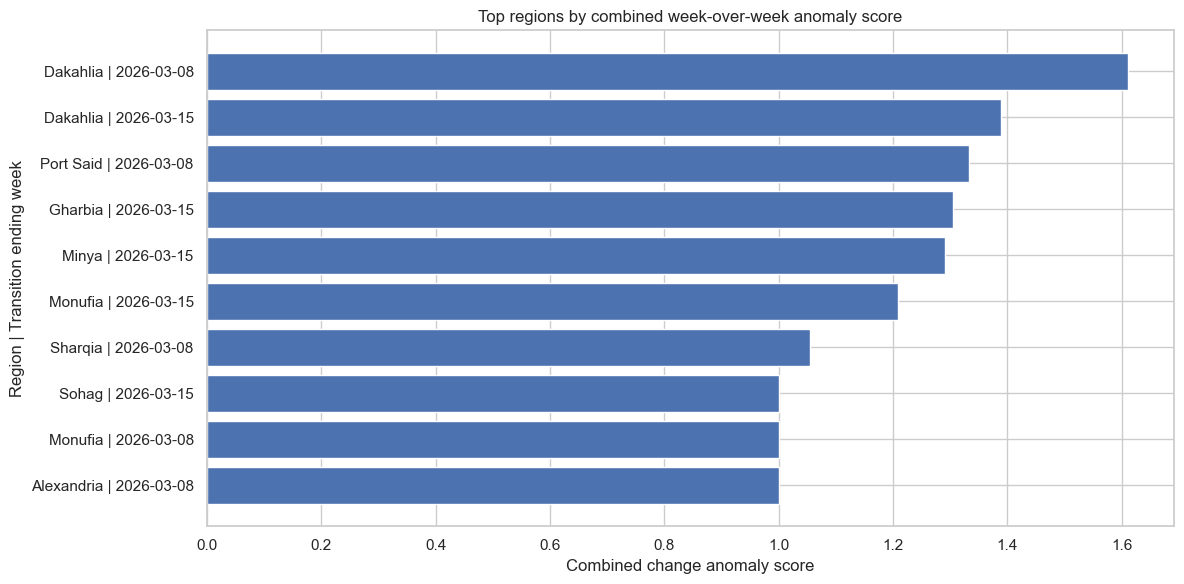
\includegraphics[width=1\linewidth]{Images/Top_regions_by_combined_week-over-week_anomaly_score.png}
    \caption{Top regions by combined week-over-week anomaly score.}
    \label{fig:combinedwow}
\end{figure}

\FloatBarrier

\subsection{Q3: Which region-carrier pairs were outliers within their region?}

The strongest peer anomalies are dominated by \textbf{Operator C on LTE}, especially in Assiut, Ismailia, Giza, Alexandria, and Gharbia. These cases combine two negative signs: download below peers and latency above peers.

\begin{table}[htbp]
\centering
\scriptsize
\begin{adjustbox}{max width=\textwidth}
\begin{tabular}{l l l l r r r}
\toprule
Week & Region & Carrier & Tech & Download gap (\%) & Latency gap (\%) & Score \\
\midrule
2026-03-08 & Assiut & Operator C & LTE & -67.46 & 70.65 & 138.11 \\
2026-03-01 & Assiut & Operator C & LTE & -52.03 & 83.96 & 135.99 \\
2026-03-15 & Assiut & Operator C & LTE & -68.50 & 66.79 & 135.29 \\
2026-03-08 & Ismailia & Operator C & LTE & -61.68 & 69.12 & 130.79 \\
2026-03-01 & Ismailia & Operator C & LTE & -61.89 & 64.37 & 126.26 \\
2026-03-01 & Alexandria & Operator C & LTE & -65.18 & 57.86 & 123.04 \\
2026-03-15 & Gharbia & Operator C & LTE & -56.64 & 63.21 & 119.86 \\
2026-03-15 & Ismailia & Operator C & LTE & -51.13 & 57.46 & 108.58 \\
\bottomrule
\end{tabular}
\end{adjustbox}
\caption{Top cross-sectional peer anomalies after applying the slide badness formula.}
\label{tab:peer}
\end{table}

\begin{figure}[htbp]
    \centering
    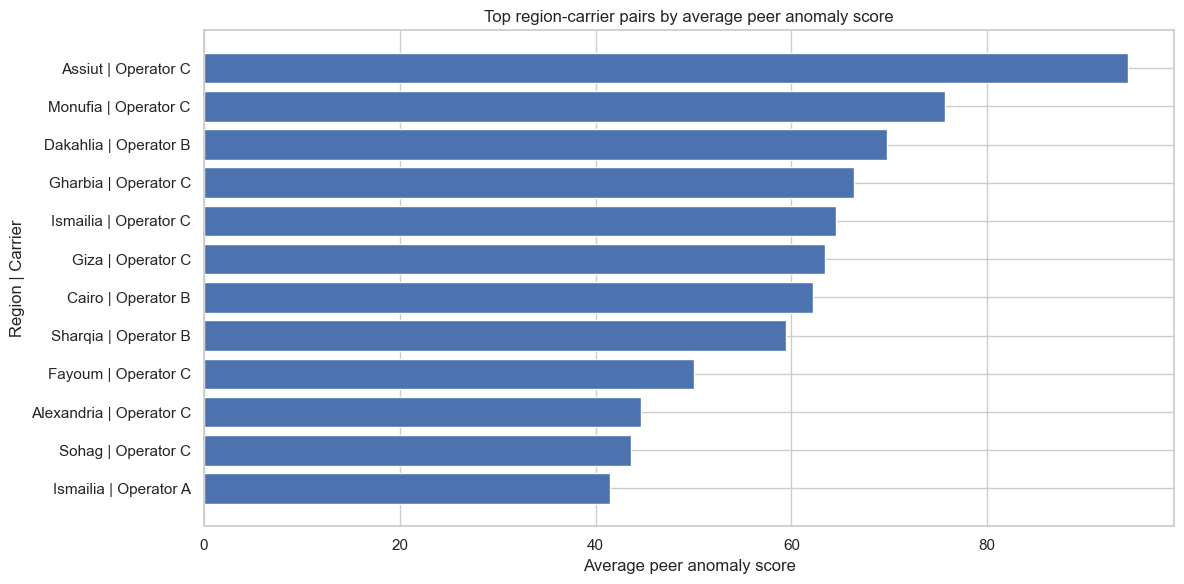
\includegraphics[width=1\linewidth]{Images/top_peer_anomalies.png}
    \caption{Top region-carrier pairs by average peer anomaly score.}
    \label{fig:peer}
\end{figure}

\FloatBarrier

\subsection{Q4: Is the 5G distribution different from LTE?}

Yes. 5G is substantially stronger than LTE across the final cleaned data.

\begin{table}[htbp]
\centering
\begin{adjustbox}{max width=\textwidth}
\begin{tabular}{lrrrr}
\toprule
Technology & Observations & Avg download (kbps) & Median download (kbps) & Avg latency (ms) \\
\midrule
5G & 39 & 295,221 & 301,663 & 31.30 \\
LTE & 39 & 48,988 & 50,830 & 38.02 \\
Multi-RAT & 39 & 105,193 & 111,827 & 35.83 \\
\bottomrule
\end{tabular}
\end{adjustbox}
\caption{Distribution summary by technology across all 39 region-week observations.}
\label{tab:tech}
\end{table}

Across all 39 region-week comparisons, 5G never underperformed LTE in median download. The average 5G-minus-LTE gap was approximately \num{246233} kbps. A stricter matched-carrier check was also performed using 109 region-week-carrier comparisons where both LTE and 5G existed. In those matched cases, 5G underperformed LTE in \textbf{0} cases.

\begin{figure}[htbp]
    \centering
    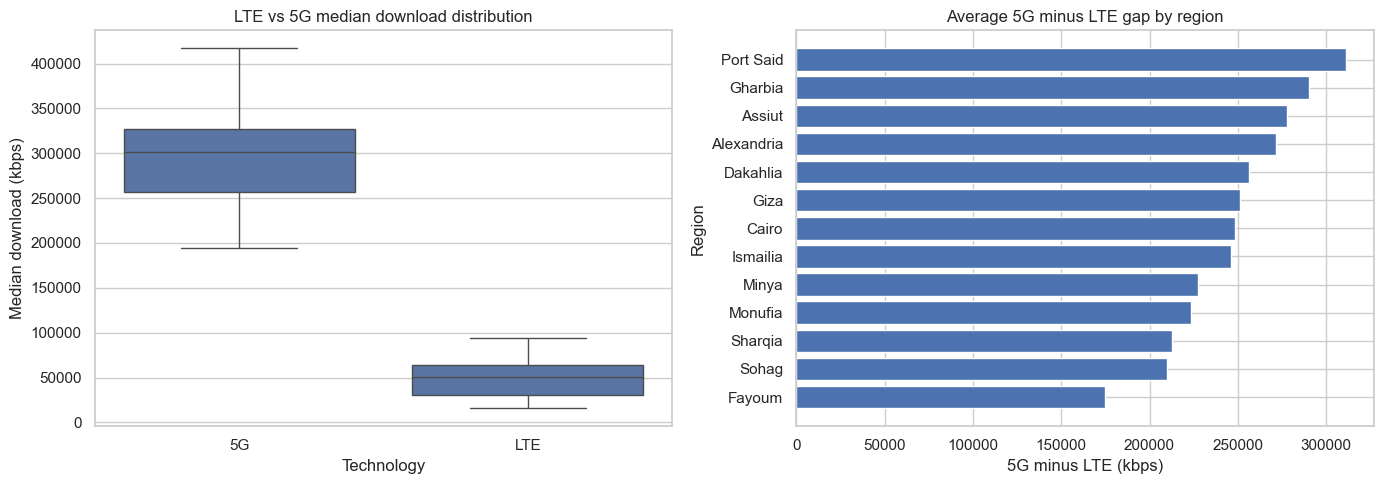
\includegraphics[width=1\linewidth]{Images/4G_vs_5G_Distribution.png}
    \caption{LTE vs 5G median download distribution and average 5G-minus-LTE gap by region.}
    \label{fig:techdist}
\end{figure}

\FloatBarrier

\subsection{Q5: Regional ranking and rank stability}

The regional ranking was built from the weighted median-download proxy after combining carriers and technologies using sample-count weights. Rank 1 is the best.

\begin{table}[htbp]
\centering
\small
\begin{adjustbox}{max width=\textwidth}
\begin{tabular}{lrrr}
\toprule
Region & 2026-03-01 & 2026-03-08 & 2026-03-15 \\
\midrule
Alexandria & 4 & 5 & 6 \\
Assiut & 3 & 2 & 3 \\
Cairo & 10 & 9 & 8 \\
Dakahlia & 9 & 10 & 10 \\
Fayoum & 12 & 11 & 11 \\
Gharbia & 2 & 1 & 2 \\
Giza & 5 & 4 & 4 \\
Ismailia & 6 & 6 & 5 \\
Minya & 7 & 8 & 9 \\
Monufia & 8 & 7 & 7 \\
Port Said & 1 & 3 & 1 \\
Sharqia & 11 & 12 & 12 \\
Sohag & 13 & 13 & 13 \\
\bottomrule
\end{tabular}
\end{adjustbox}
\caption{Regional ranking based on aggregated median download speed proxy (1 = best).}
\label{tab:rank}
\end{table}

The strongest regions were generally \textbf{Port Said}, \textbf{Gharbia}, and \textbf{Assiut}. The weakest were consistently \textbf{Sohag}, \textbf{Sharqia}, and \textbf{Fayoum}. Sohag remained rank 13 in all three weeks, which makes it weak but stable. The most unstable region was \textbf{Port Said}, whose rank moved from 1 to 3 and back to 1.

\begin{table}[htbp]
\centering
\begin{adjustbox}{max width=\textwidth}
\begin{tabular}{lrr}
\toprule
Region & Rank range & Total absolute rank movement \\
\midrule
Port Said & 2 & 4 \\
Alexandria & 2 & 2 \\
Cairo & 2 & 2 \\
Minya & 2 & 2 \\
Assiut & 1 & 2 \\
\bottomrule
\end{tabular}
\end{adjustbox}
\caption{Most unstable regions by ranking movement.}
\label{tab:unstable}
\end{table}

\begin{figure}[htbp]
    \centering
    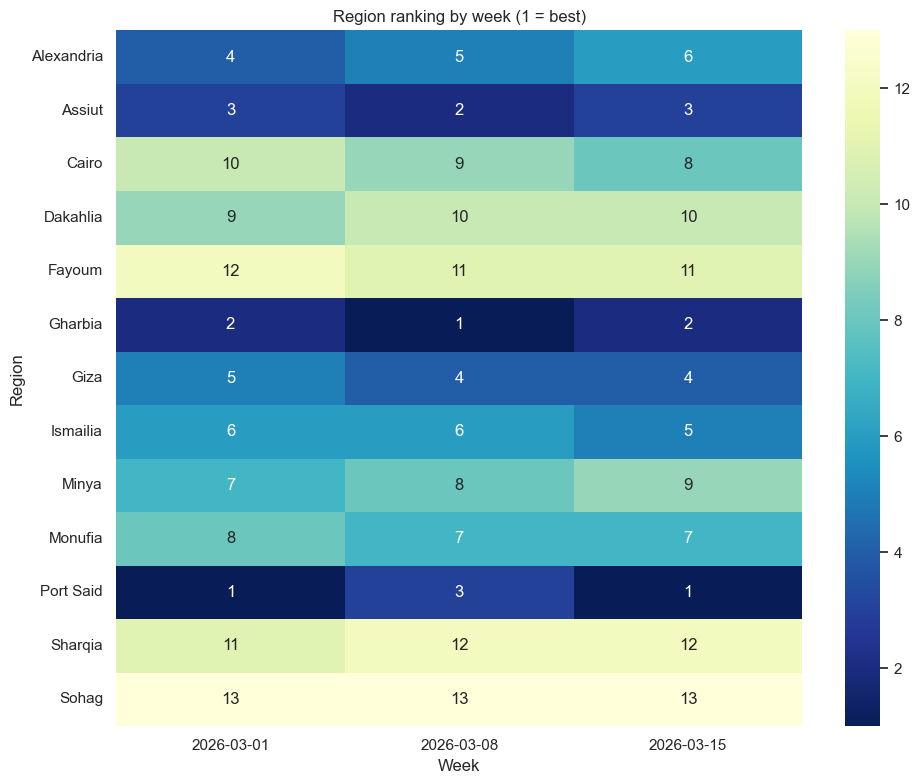
\includegraphics[width=0.9\linewidth]{Images/region_rank_trajectories.png}
    \caption{Regional rank trajectories across the three weekly snapshots (1 = best).}
    \label{fig:rank}
\end{figure}

\FloatBarrier

\section{Additional Required Deliverables}

\subsection{Carrier report}

The carrier report compares Operators A, B, and C across regions and weeks. The final version separates two different meanings of ``worst carrier'':

\begin{itemize}
    \item \textbf{Worst by download:} the carrier with the lowest average weighted median-download proxy in the region.
    \item \textbf{Worst by peer anomaly score:} the carrier with the highest average cross-sectional badness score in the region.
\end{itemize}

This separation is important because a carrier can have the lowest absolute download in a region without being the largest relative peer anomaly.

\begin{table}[htbp]
\centering
\small
\begin{adjustbox}{max width=\textwidth}
\begin{tabular}{l l l r}
\toprule
Region & Worst by download & Worst by peer score & Avg peer score \\
\midrule
Alexandria & Operator A & Operator C & 44.66 \\
Assiut & Operator A & Operator C & 94.35 \\
Cairo & Operator B & Operator B & 62.24 \\
Dakahlia & Operator B & Operator B & 69.73 \\
Fayoum & Operator C & Operator C & 50.09 \\
Gharbia & Operator A & Operator C & 66.41 \\
Giza & Operator A & Operator C & 63.47 \\
Ismailia & Operator A & Operator C & 64.51 \\
Minya & Operator A & Operator A & 20.51 \\
Monufia & Operator C & Operator C & 75.70 \\
Port Said & Operator A & Operator B & 17.37 \\
Sharqia & Operator B & Operator B & 59.46 \\
Sohag & Operator C & Operator C & 43.60 \\
\bottomrule
\end{tabular}
\end{adjustbox}
\caption{Worst carrier per region under two definitions.}
\label{tab:worst}
\end{table}

\subsection{Anomaly logs}

Three CSV deliverables were generated for reproducibility and presentation use:

\begin{enumerate}[label=\arabic*.]
    \item \texttt{project6\_peer\_anomaly\_log.csv}
    \item \texttt{project6\_change\_anomaly\_log.csv}
    \item \texttt{project6\_anomaly\_log.csv} (combined log)
\end{enumerate}

The combined anomaly log contains 20 flagged rows: 17 cross-sectional peer anomalies and 3 week-over-week change anomalies.

\subsection{Mean vs median analysis}

Project 6 asks for an explanation of where mean and median diverge. Large positive gaps between mean and median often suggest a right-skewed distribution, where a few unusually high values pull the mean upward. For latency, a large mean above the median suggests a tail of unusually poor high-latency measurements.

\begin{table}[htbp]
\centering
\scriptsize
\begin{adjustbox}{max width=\textwidth}
\begin{tabular}{l l l l l r r r}
\toprule
Week & Region & Carrier & Tech & Metric & Mean & Median proxy & Gap (\%) \\
\midrule
2026-03-01 & Sohag & Operator B & Multi-RAT & Download & 85,102.58 & 22,048.46 & 285.98 \\
2026-03-08 & Sohag & Operator B & Multi-RAT & Download & 77,237.58 & 25,142.46 & 207.20 \\
2026-03-01 & Port Said & Operator C & 5G & Latency & 25.25 & 16.44 & 53.57 \\
2026-03-08 & Cairo & Operator C & LTE & Latency & 54.42 & 35.77 & 52.13 \\
\bottomrule
\end{tabular}
\end{adjustbox}
\caption{Illustrative cases where mean and median diverge strongly.}
\label{tab:mm}
\end{table}

\begin{figure}[htbp]
    \centering
    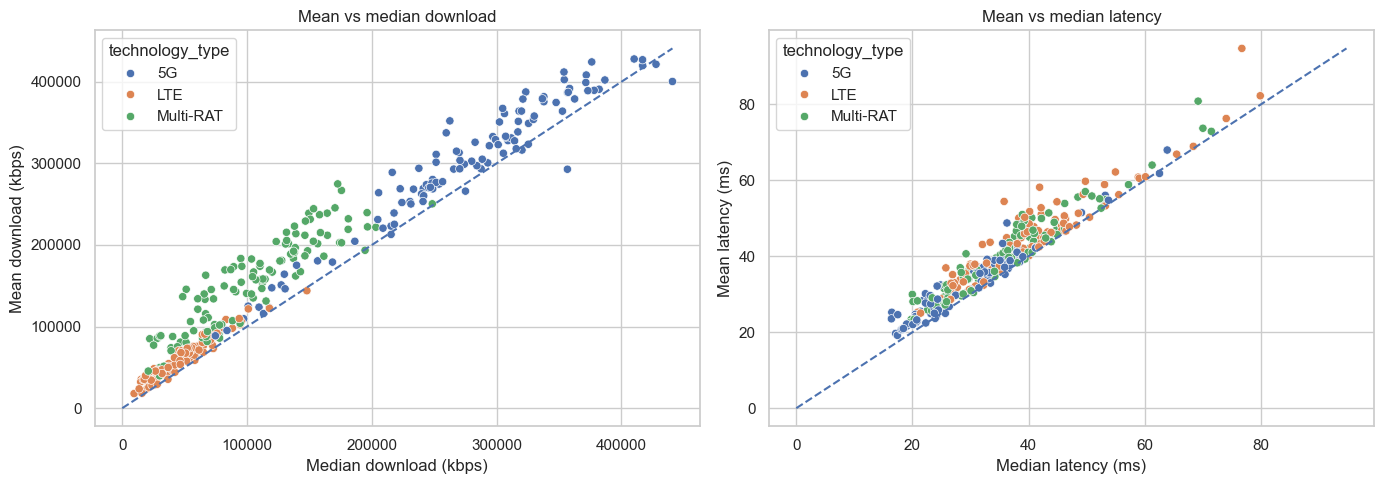
\includegraphics[width=1\linewidth]{Images/mean_vs_median.png}
    \caption{Mean vs median comparison for download and latency.}
    \label{fig:mm}
\end{figure}

\FloatBarrier

\section{Limitations}

The workflow is strong and appropriate for Project 6, but the following limitations should be remembered:

\begin{itemize}
    \item The dataset contains only three weekly snapshots, so long-history temporal models such as rolling baselines, CUSUM, EWMA, or sequence models are not appropriate as primary methods.
    \item Median KPIs are \textbf{weighted proxies} derived from locality medians, not exact combined medians from raw speed-test records.
    \item The analysis is descriptive and anomaly-oriented. It identifies suspicious patterns but does not prove physical root cause.
    \item The threshold \texttt{sample\_count\_total >= 30} is a balanced choice for this dataset. It improves coverage compared with 50, but still removes the weakest region-carrier-technology-week rows.
    \item Complete peer-group filtering improves fairness for Q1 and Q3, but it excludes 13 rows that do not have all three carriers available in the same region-week-technology peer group.
\end{itemize}

\section{Conclusion}

The final corrected workflow produced a complete and explainable Project 6 solution. The most important conclusions are:

\begin{itemize}
    \item \textbf{Operator C} is the main consistent underperformer relative to regional peers. Operator B is slightly below the weighted peer baseline but is much less severe and nearly neutral by the final week.
    \item The largest direct download drops were concentrated in \textbf{Assiut}, \textbf{Monufia}, \textbf{Gharbia}, \textbf{Minya}, and \textbf{Alexandria}.
    \item The strongest combined week-over-week anomalies were led by \textbf{Dakahlia} and \textbf{Port Said}.
    \item The strongest peer anomalies were repeatedly driven by \textbf{Operator C on LTE}, especially in Assiut, Ismailia, Giza, Alexandria, and Gharbia.
    \item \textbf{5G clearly outperformed LTE} across all region-week comparisons and all matched carrier-level comparisons.
    \item \textbf{Port Said} was the most unstable region by rank movement, while \textbf{Sohag} remained the weakest but stable bottom-ranked region.
\end{itemize}

\section{Changes Compared with the First Report Version}

The final report differs from the first version in the following important ways:

\begin{enumerate}[label=\arabic*.]
    \item \textbf{Date parsing was corrected.} The earlier two-week issue was caused by forcing day-first parsing on ISO-formatted dates. The final notebooks preserve all three weeks.
    \item \textbf{The sample threshold changed from 50 to 30.} This increased the final cleaned table from 335 to 343 rows and raised complete peer-comparison coverage from 312 to 330 rows.
    \item \textbf{The peer anomaly score now exactly matches the slide formula.} The score is no longer a percentile-rank score; it is the sum of download underperformance and latency overperformance in bad percentage-gap points.
    \item \textbf{Complete peer-group filtering was added.} Q1 and Q3 now use only groups where all three carriers are present.
    \item \textbf{Q2 was split into direct KPI changes and combined anomaly score.} The report now distinguishes largest download drops, largest latency rises, and combined week-over-week anomaly flags.
    \item \textbf{The carrier report now separates worst-by-download from worst-by-peer-score.} This avoids mixing absolute weakness with relative anomaly severity.
    \item \textbf{The 5G-vs-LTE section now includes a matched-carrier validation.} This confirms that 5G underperformed LTE in zero matched carrier-region-week cases.
    \item \textbf{All tables were refreshed from the final generated CSV outputs.} The report tables now match the corrected preprocessing and analysis notebooks.
\end{enumerate}

\section*{Appendix: Generated Files}

The report was built alongside the following main outputs:

\begin{itemize}
    \item \texttt{weekly\_locality\_only.csv}
    \item \texttt{weekly\_country\_only.csv}
    \item \texttt{weekly\_region\_carrier\_tech.csv}
    \item \texttt{project6\_carrier\_report.csv}
    \item \texttt{project6\_peer\_anomaly\_log.csv}
    \item \texttt{project6\_change\_anomaly\_log.csv}
    \item \texttt{project6\_anomaly\_log.csv}
    \item \texttt{project6\_region\_ranking.csv}
    \item \texttt{project6\_rank\_stability.csv}
    \item \texttt{project6\_fiveg\_vs\_lte.csv}
    \item \texttt{project6\_fiveg\_vs\_lte\_matched\_carrier.csv}
    \item \texttt{project6\_mean\_median\_examples.csv}
\end{itemize}

\end{document}
